\section{Experiments}  \label{Experiments}

In this section, we first present a comparative analysis of the proposed model on the video object detection task. Second, we present an ablation study analyzing the effects of different training procedures on the robustness of the model to sensor failure scenarios.

\subsection{Training for Bounding Boxes} \label{Experiments:TrainingBoundingBoxes}

We train the RPerceiver with used AdamW optimizer \cite{loshchilovDecoupledWeightDecay2019a} setting the initial learning rates for the movel $ 10^{-4} $. We trained for 31 epochs with a learning rate drop by a factor of 10 at epoch 18 and 28. Data augmentation pipeline includes normalization based on pre-calculated dataset statistics, and frames are resized to a fixed dimension 320 x 320 \cite{redmonYOLO9000BetterFaster2016}. Other training hyperparameters can be found in section \ref{Appendix:TrainingHyperparameters}.

\subsection{Comparison Analysis} \label{Experiments:ComparisonAnalysis}

First, we consider the task of object detection using the detection-moving-mnist-easy benchmark from Section \ref{Methods:Dataset}. We perform a comparative analysis against a still-image object detector of comparable size, YOLOv8n \cite{Jocher_Ultralytics_YOLO_2023}. The primary goal is to evaluate how the proposed RPerceiver architecture utilizes spatio-temporal information from the video input. Results are shown in Table \ref{tab:model_comparison}.

% YOLO: Raw mAP Results (Evaluator): {'map': tensor(0.9231), 'map_50': tensor(0.9621), 'map_75': tensor(0.9410), 'map_small': tensor(0.9231), 'map_medium': tensor(-1.), 'map_large': tensor(-1.), 'mar_1': tensor(0.7471), 'mar_10': tensor(0.9393), 'mar_100': tensor(0.9393), 'mar_small': tensor(0.9393), 'mar_medium': tensor(-1.), 'mar_large': tensor(-1.), 'map_per_class': tensor(-1.), 'mar_100_per_class': tensor(-1.), 'classes': tensor([0, 1, 2, 3, 4, 5, 6, 7, 8, 9], dtype=torch.int32)}

% RPerceiver: Raw mAP Results (Evaluator): {'map': tensor(0.9025), 'map_50': tensor(0.9688), 'map_75': tensor(0.9442), 'map_small': tensor(0.9025), 'map_medium': tensor(-1.), 'map_large': tensor(-1.), 'mar_1': tensor(0.7367), 'mar_10': tensor(0.9240), 'mar_100': tensor(0.9240), 'mar_small': tensor(0.9240), 'mar_medium': tensor(-1.), 'mar_large': tensor(-1.), 'map_per_class': tensor(-1.), 'mar_100_per_class': tensor(-1.), 'classes': tensor([0, 1, 2, 3, 4, 5, 6, 7, 8, 9], dtype=torch.int32)}

% TODO: recompute GFLOPS

\begin{table}[htb!]
    \centering
    \caption{Comparison with the baseline still image detector YOLOv8n \cite{Jocher_Ultralytics_YOLO_2023} on the detection-moving-mnist-easy test split. 'Post' indicates the use of postprocessing heuristics. RPerceiver achieves slightly better $mAP_{50}$ and $mAP_{75}$, but shows worse $mAP_{50-95}$ results. However, RPerceiver achieves these results with significantly fewer parameters and lower computational cost.}
    \label{tab:model_comparison}
    \begin{tblr}{width=1\textwidth, hlines, vlines,
                  colspec = { l c c c c c c },
                  row{1} = {font=\bfseries},
                 }
        Model      & Post & mAP_{50} & mAP_{75} & mAP_{50-95} & Params (M)   & GFLOPS         \\
        YOLOv8n    & X & 96.2  & 94.1 & \textbf{92.3}  & 3            & 8.1            \\
        RPerceiver & X & \textbf{96.9} & \textbf{94.4} & 90.3 &\textbf{1} & \textbf{1.2}   \\
    \end{tblr}
\end{table}

\begin{figure}
    \centering
    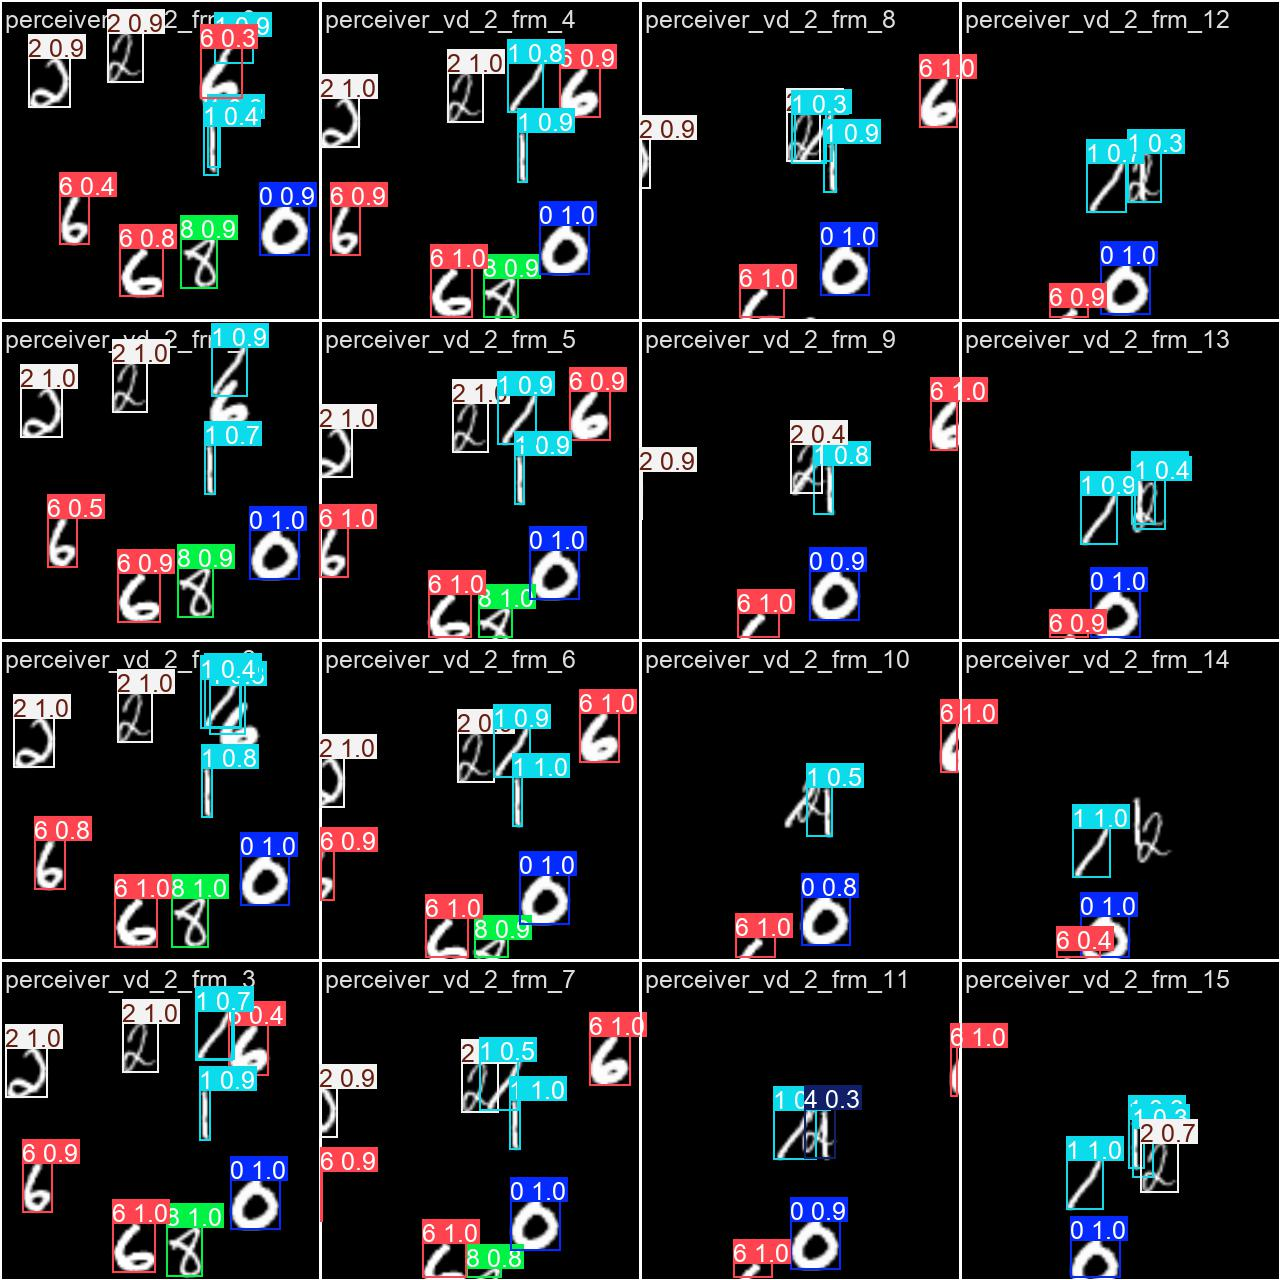
\includegraphics[width=\textwidth]{figures/figure_methods_val_batch2_pred_recurrent_perceiver.jpg}
    \caption{Visualization of RPerceiver predictions across sequential frames. Bounding boxes and confidence scores are displayed for detected digits. Notably, confidence scores can be less than 1.0 even for clear objects (e.g. digits in frame 1). Two challenging scenarios are analyzed: overlapping digits and digits near the frame border. The model shows limitations such as exhibiting false negatives with overlapping digits, as illustrated by the central cluster involving digits such as '1's and a '2' between frames 8 and 15. In contrast, predictions appear consistent between frames 5 and 13 for several digits near frame borders: the '2' and '6' on the left border, the '6' and '8' near the bottom border, and the '6' on the right border.}
    \label{fig:figure_methods_val_batch2_pred_recurrent_perceiver}
\end{figure}

\begin{figure}
    \centering
    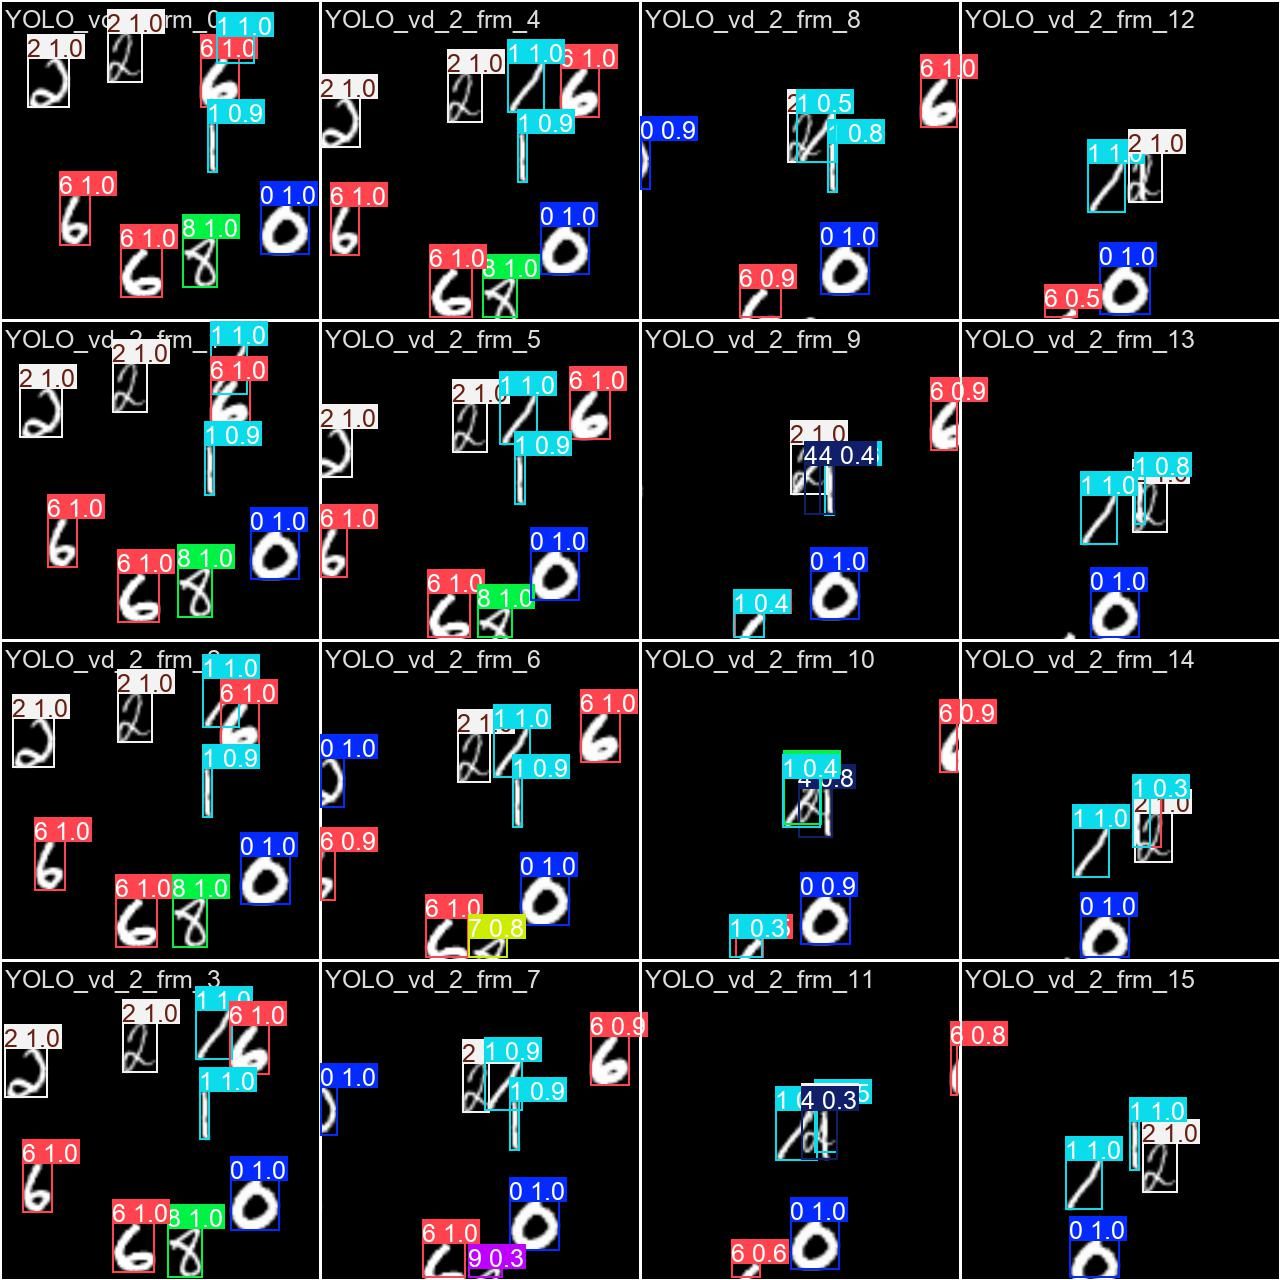
\includegraphics[width=\textwidth]{figures/figure_methods_val_batch2_pred_YOLO.jpg}
    \caption{Visualization of YOLOv8n \cite{Jocher_Ultralytics_YOLO_2023} predictions across sequential frames. Bounding boxes and confidence scores are displayed for detected digits. Notably, confidence scores are typically high (often 1.0) for relatively clear objects (e.g., digits in frame 1). Two challenging scenarios are analyzed: overlapping digits and digits near the frame border. The model appears to handle overlapping digits relatively effectively, with a few false negatives in the central cluster involving digits such as '1's and a '2' between frames 8 and 15. In contrast, predictions appear inconsistent between frames 5 and 13 for several digits near frame borders: the '2' on the left border, the '6' and '8' near the bottom border.}
    \label{fig:figure_methods_val_batch2_pred_YOLO}
\end{figure}

% TODO: recompute with tighter IoU threshold

To quantify the observations regarding model performance in challenging scenarios, as illustrated in Figures \ref{fig:figure_methods_val_batch2_pred_recurrent_perceiver} and \ref{fig:figure_methods_val_batch2_pred_YOLO}, we specifically evaluated the models on filtered subsets of the ground truth data. These subsets isolate two challenging conditions: overlapping objects (defined as pairs of ground truth objects with an Intersection over Union (IoU) greater than 0.01) and border objects (defined as ground truth objects whose bounding boxes intersect with the frame border). The resulting performance metrics for these specific cases are presented in Table \ref{tab:model_comparison_detailed}.

% YOLO:
% Raw Overlap mAP Results (Evaluator): {'map': tensor(0.8266), 'map_50': tensor(0.9133), 'map_75': tensor(0.8788), 'map_small': tensor(0.8266), 'map_medium': tensor(-1.), 'map_large': tensor(-1.), 'mar_1': tensor(0.7744), 'mar_10': tensor(0.8536), 'mar_100': tensor(0.8536), 'mar_small': tensor(0.8536), 'mar_medium': tensor(-1.), 'mar_large': tensor(-1.), 'map_per_class': tensor(-1.), 'mar_100_per_class': tensor(-1.), 'classes': tensor([0, 1, 2, 3, 4, 5, 6, 7, 8, 9], dtype=torch.int32)}

% Raw Boundary mAP Results (Evaluator): {'map': tensor(0.6989), 'map_50': tensor(0.7667), 'map_75': tensor(0.7365), 'map_small': tensor(0.6989), 'map_medium': tensor(-1.), 'map_large': tensor(-1.), 'mar_1': tensor(0.7119), 'mar_10': tensor(0.7280), 'mar_100': tensor(0.7280), 'mar_small': tensor(0.7280), 'mar_medium': tensor(-1.), 'mar_large': tensor(-1.), 'map_per_class': tensor(-1.), 'mar_100_per_class': tensor(-1.), 'classes': tensor([0, 1, 2, 3, 4, 5, 6, 7, 8, 9], dtype=torch.int32)}

% RPerceiver
% Raw Overlap mAP Results (Evaluator): {'map': tensor(0.6940), 'map_50': tensor(0.8853), 'map_75': tensor(0.7777), 'map_small': tensor(0.6940), 'map_medium': tensor(-1.), 'map_large': tensor(-1.), 'mar_1': tensor(0.6686), 'mar_10': tensor(0.7389), 'mar_100': tensor(0.7389), 'mar_small': tensor(0.7389), 'mar_medium': tensor(-1.), 'mar_large': tensor(-1.), 'map_per_class': tensor(-1.), 'mar_100_per_class': tensor(-1.), 'classes': tensor([0, 1, 2, 3, 4, 5, 6, 7, 8, 9], dtype=torch.int32)}

% Raw Boundary mAP Results (Evaluator): {'map': tensor(0.8470), 'map_50': tensor(0.9552), 'map_75': tensor(0.9101), 'map_small': tensor(0.8470), 'map_medium': tensor(-1.), 'map_large': tensor(-1.), 'mar_1': tensor(0.8512), 'mar_10': tensor(0.8739), 'mar_100': tensor(0.8739), 'mar_small': tensor(0.8739), 'mar_medium': tensor(-1.), 'mar_large': tensor(-1.), 'map_per_class': tensor(-1.), 'mar_100_per_class': tensor(-1.), 'classes': tensor([0, 1, 2, 3, 4, 5, 6, 7, 8, 9], dtype=torch.int32)}


\begin{table}[htb!]
    \centering
    \caption{Comparative analysis of YOLOv8n \cite{Jocher_Ultralytics_YOLO_2023} and RPerceiver on specific scenarios within the detection-moving-mnist-easy test split: object overlaps ('Overlap') and proximity to image borders ('Border'). Postprocessing ('Post') is applied to both models. The data indicates that the still-image detector YOLOv8n achieves higher accuracy on overlapping objects. In contrast, RPerceiver significantly outperforms YOLOv8n on border cases, supporting the hypothesis that it effectively leverages temporal information from the video sequence.}
\label{tab:model_comparison_detailed}

    \label{tab:model_comparison_detailed}
    \begin{tblr}{width=1\textwidth, hlines, vlines,
                  colspec = { l c c c c c },
                  row{1} = {font=\bfseries},
                 }
        \SetCell[r=2]{l}Model & \SetCell[r=2]{l}Post & \SetCell[c=3]{c}Overlap & & & \SetCell[c=3]{c}Border & & \\
                   &   & mAP_{50} & mAP_{75}  & mAP_{50-95}       & mAP_{50} & mAP_{75}  & mAP_{50-95}  \\
        YOLOv8n    & X & \textbf{91.3}  & \textbf{87.9} & \textbf{82.7} & 76.7  & 73.7 & 69.9 \\
        RPerceiver & X & 88.5 & 77.8 & 69.4  & \textbf{95.5} & \textbf{91.0} & \textbf{84.7}\\
    \end{tblr}
\end{table}

\subsection{Ablation Study} \label{Experiments:AblationStudy}

In this ablation study, we evaluate the robustness of the RPerceiver and RPerceiverMM models against complete sensor failure and non-deterministic sensor input. The evaluation employs the center point prediction task. We experimented with two primary configurations: \texttt{single-view} and \texttt{multi-view}. First, the \texttt{single-view} configuration utilized a single camera sensor, representing a basic object detection task using video input. Second, the \texttt{multi-view} setting involved processing information from multiple cameras to perform object detection within a unified spatial representation derived from these inputs.

We considered three distinct evaluation procedures: \texttt{default}, \texttt{shuffle}, and \texttt{blind}. Additionally, we evaluated a combination of the latter two procedures.

\begin{description}
    \item[\texttt{default}] This procedure represents the normal operational regime where all sensors function as expected without any induced faults or input shuffle.

    \item[\texttt{shuffle}] In this procedure, the sensor inputs are randomly permuted within each time step. Consequently, the model receives inputs from the sensors in a random order for that specific time step. Shuffling occurs only for sensor inputs within the same time step. This procedure is applicable only to the \texttt{multi-view} setup.

    \item[\texttt{blind}] This procedure simulates a complete sensor(s) failure scenario where the input from camera sensor(s) becomes unavailable. The \texttt{blind} procedure is implemented by dropping the input stream from the sensor(s) after a midpoint time step, $t_{half}$. Consequently, information from the sensor(s) is unavailable to the model for the second half of the sequence.
\end{description}

It is important to note the conceptual link between the \texttt{dropout} training procedure described in Section \ref{Methods:DropoutAndShuffle} and the \texttt{blind} evaluation procedure defined here. The \texttt{blind} procedure can be viewed as a specific, deterministic instance of the \texttt{dropout} mechanism applied during evaluation. Specifically, it corresponds to a scenario where the probability of dropping the sensor input becomes 1.0. While \texttt{dropout} during training introduces stochasticity with varying probabilities to enhance general robustness, the \texttt{blind} evaluation tests the model's resilience to a complete and sustained sensor failure.

We initiate our analysis by comparing the performance of the baseline RPerceiver (RP) model against its counterpart trained using the dropout procedure (RP (d)), as described in Section \ref{Methods:DropoutAndShuffle}. This comparison is conducted under the \texttt{single-view} configuration using the \texttt{default} evaluation procedure. The results of this evaluation are presented in Table~\ref{tab:results_single_view_default}.

\begin{table}[htb!]
    \centering
    \caption{Comparison of RPerceiver (RP) and RPerceiver trained with dropout (RP (d)) under the \texttt{single-view} configuration and \texttt{default} evaluation procedure. The '(d)' denotes training with dropout. Results are presented based on the number of digits in the input sequence. Metrics shown are Average Displacement Error (ADE), calculated over the second half of the sequence, and Final Displacement Error (FDE), calculated for the final frame. The results indicate that the baseline RPerceiver consistently outperforms the RPerceiver trained with dropout, achieving lower error rates for both ADE and FDE across all tested sequence complexities.
    }
    \label{tab:results_single_view_default}
    \begin{tblr}{width=1\textwidth, hlines, vlines,
                    colspec = { l c c c c c c c c c c },
                    row{1} = {font=\bfseries},
                    row{2} = {font=\bfseries},
                }
        \SetCell[r=2]{l} Model & \SetCell[c=2]{c}1 digit & & \SetCell[c=2]{c}2 digits & & \SetCell[c=2]{c}4 digits & & \SetCell[c=2]{c}8 digits & & \SetCell[c=2]{c}10 digits & \\
        & ADE & FDE & ADE & FDE & ADE & FDE & ADE & FDE & ADE & FDE \\
        RP              & \textbf{0.717} & \textbf{0.725} & \textbf{0.794} & \textbf{0.793} & \textbf{0.958} & \textbf{0.934} & \textbf{1.520} & \textbf{1.382} & \textbf{3.273} & \textbf{2.611} \\
        RP (d) & 0.745 & 0.793 & 0.838 & 0.882 & 1.034 & 1.065 & 1.656 & 1.583 & 3.626 & 3.12 \\
    \end{tblr}
\end{table}

Next, we compare the same models, RPerceiver (RP) and RPerceiver trained with dropout (RP (d)). This comparison is conducted under the \texttt{single-view} configuration using the \texttt{blind} evaluation procedure. The results for this \texttt{blind} test are detailed in Table~\ref{tab:results_frame_dropout_blind}.

\begin{table}[htb!]
    \centering
    \caption{Comparison of RPerceiver (RP) and RPerceiver trained with dropout (RP (d)) under the \texttt{single-view} configuration and \texttt{blind} evaluation procedure. The '(d)' denotes training with dropout. Results are presented based on the number of digits in the input sequence. Metrics shown are Average Displacement Error (ADE), calculated over the second half of the sequence, and Final Displacement Error (FDE), calculated for the final frame. The results under the \texttt{blind} condition demonstrate a significant advantage for the RPerceiver trained with dropout (RP (d)). This model maintains substantially lower error rates compared to the baseline RP, which exhibits a sharp degradation in performance under the \texttt{blind} evaluation procedure.
    }
    \label{tab:results_frame_dropout_blind}
    \begin{tblr}{width=1\textwidth, hlines, vlines,
                    colspec = { l c c c c c c c c c c },
                    row{1} = {font=\bfseries},
                    row{2} = {font=\bfseries},
                    colsep=3pt,
                }
        \SetCell[r=2]{l} Model & \SetCell[c=2]{c}1 digit & & \SetCell[c=2]{c}2 digits & & \SetCell[c=2]{c}4 digits & & \SetCell[c=2]{c}8 digits & & \SetCell[c=2]{c}10 digits & \\
        & ADE & FDE & ADE & FDE & ADE & FDE & ADE & FDE & ADE & FDE \\
        RP              & 42.210 & 34.754 & 36.087 & 28.83014 & 32.146 & 24.397 & 31.32972 & 23.730 & 33.334 & 25.935 \\
        RP (d)             & \textbf{1.541} & \textbf{1.101} & \textbf{1.907} & \textbf{1.364} & \textbf{2.658} & \textbf{1.905} & \textbf{5.084} & \textbf{3.679} & \textbf{8.198} & \textbf{6.627} \\
    \end{tblr}
\end{table}

For the \texttt{multi-view} configuration, we introduce a tile augmentation technique to the dataset pipeline. This process divides each frame into a specified grid of views, partitioning the corresponding ground truths as well. In our experiments, we utilize a $2 \times 2$ grid configuration. This effectively treats the tiled frame as a simplified spatial layout, akin to a Bird's-Eye View (BEV) where each tile represents a spatial region. Figure~\ref{fig:figure_methods_dataset_image_view_bev} illustrates an example of a frame divided using this grid approach.

\begin{figure}
    \centering
    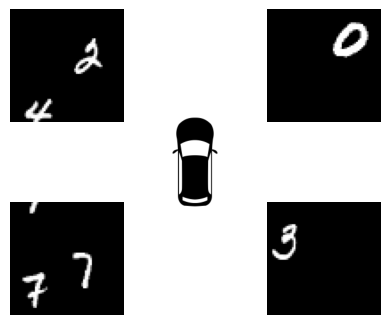
\includegraphics[width=0.33\textwidth]{figures/figure_methods_dataset_image_view_bev.png}
    \caption{Bird Eye View (BEV) of the frame raster divided into grid.}
    \label{fig:figure_methods_dataset_image_view_bev}
\end{figure}

We now extend our ablation study to the \texttt{multi-view} configuration, evaluating the RPerceiverMM (RPMM) model and its variants trained with training procedures from Section \ref{Methods:DropoutAndShuffle}: shuffle training (RPMM (s)), dropout training (RPMM (d)), and combined shuffle and dropout training (RPMM (d, s)). These models are compared against the baseline RPMM under four distinct evaluation procedures: \texttt{default}, \texttt{shuffle}, \texttt{blind}, and a combined \texttt{blind} and \texttt{shuffle} scenario. The performance metrics for these multi-view evaluations are presented in Table~\ref{tab:results_multi_view}.

% Results: https://docs.google.com/spreadsheets/d/1shITm2iWIKzAAlWpRwED-g1H6YurMJoJgxagRU2x6Gg/edit?gid=290835343#gid=290835343

\begin{table}[htb!]
    \centering
    \caption{Comparison of RPerceiverMM (RPMM) variants under the \texttt{multi-view} configuration across different evaluation procedures: \texttt{default}, \texttt{shuffle}, \texttt{blind}, and combined \texttt{blind, shuffle}. Model notations indicate training procedures: '(s)' for shuffle training, '(d)' for dropout training, and '(d, s)' for combined dropout and shuffle training. Metrics shown are Average Displacement Error (ADE), calculated over the second half of the sequence, Final Displacement Error (FDE), calculated for the final frame, and the number of model parameters in millions (Params (M)). The results highlight trade-offs: baseline RPMM performs best under \texttt{default} conditions. While these training procedures introduce a small performance penalty in the \texttt{default} evaluation, they provide substantial improvements under performance-degrading evaluation strategies. Models trained with shuffle (s) excel in the \texttt{shuffle} evaluation, while dropout-trained models (d) show superior robustness in the \texttt{blind} scenario. The combined training (d, s) yields the most robust performance under the combined \texttt{blind, shuffle} condition, demonstrating the effectiveness of targeted training strategies for specific failure modes. Interestingly, RPMM (d) also shows notable robustness under the \texttt{shuffle} evaluation, despite not being explicitly trained for this condition.
    }
    \label{tab:results_multi_view}
    \begin{tblr}{
        hlines, vlines,
        colspec={l c c c c c c c c c},
        row{1}={font=\bfseries},
        row{2}={font=\bfseries},
    }
        \SetCell[r=2]{l}Model & \SetCell[c=2]{c}Default & & \SetCell[c=2]{c}Shuffle & & \SetCell[c=2]{c}Blind & & \SetCell[c=2]{c}Blind, Shuffle & & \SetCell[r=2]{l}{Params \\ (M)} \\
        & ADE & FDE & ADE & FDE & ADE & FDE & ADE & FDE &\\
        RPMM & 0.760 & 0.753 & 23.701 & 23.759 & 17.952 & 25.568 & 25.559 & 24.696 & 1.2 \\
        RPMM (s) & 0.823 & 0.814 & 0.812 & 0.799 & 13.644 & 20.124 & 13.670 & 20.080 & 1.2 \\
        RPMM (d) & 0.881 & 0.937 & 4.043 & 4.345 & 1.471 & 2.093 & 5.648 & 7.341 & 1.2 \\
        RPMM (d, s) & 1.073 & 1.152 & 0.956 & 1.022 & 1.729 & 2.345 & 1.632 & 2.287 & 1.2 \\
    \end{tblr}
\end{table}
